\documentclass{article}

\usepackage{amsmath,amssymb}
\usepackage{tikz}
\usepackage{xcolor}
\usepackage[left=2.1cm,right=3.1cm,bottom=3cm,footskip=0.75cm,headsep=0.5cm]{geometry}
\usepackage{enumerate}
\usepackage{enumitem}
\usepackage{marvosym}
\usepackage{tabularx}

\usepackage[utf8]{inputenc}

\renewcommand*{\arraystretch}{1.4}

\newcolumntype{L}[1]{>{\raggedright\arraybackslash}p{#1}}
\newcolumntype{R}[1]{>{\raggedleft\arraybackslash}p{#1}}
\newcolumntype{C}[1]{>{\centering\let\newline\\\arraybackslash\hspace{0pt}}m{#1}}

\title{\textbf{Einführung in die Informatik, Übung 10}}
\author{\textsc{Henry Haustein}}
\date{}

\begin{document}
	\maketitle
	
	\section*{Aufwärmübung}
	\begin{enumerate}[label=(\alph*)]
		\item $L(G_1)\cup L(G_2)$: \textcolor{blue}{$(N_1\cup N_2\cup \{S\},\Sigma,P_1\cup P_2\cup \{S\to S_1,S\to S_2\},S)$} \\
		$L(G_3)^\ast$: \textcolor{red}{$(N_3\cup \{T\},\Sigma,P_3\cup \{T\to\varepsilon,T\to TS_3\},T)$} \\
		$(L(G_1)\cup L(G_2))\cdot L(G_3)^\ast$: (\textcolor{blue}{$N_1\cup N_2\cup \{S\}$} $\cup$ \textcolor{red}{$N_3\cup \{T\}$} $\cup \,\,\{A\},\Sigma$,\textcolor{blue}{$\,P_1\cup P_2\cup \{S\to S_1,S\to S_2\}$} $\cup$ \textcolor{red}{$P_3\cup \{T\to\varepsilon,T\to TS_3\}$} $\cup \,\,\{A\to ST\},A$)
		\item $L(G_1)\cup L(G_2)$: \textcolor{blue}{$(N_1\cup N_2\cup \{S\},\Sigma,P_1\cup P_2\cup \{S\to S_1,S\to S_2\},S)$} \\
		$(L(G_1)\cup L(G_2))\cup L(G_3)$: (\textcolor{blue}{$N_1\cup N_2\cup \{S\}$} $\cup \,\,N_3\cup \{T\},\Sigma,$\textcolor{blue}{$\,P_1\cup P_2\cup \{S\to S_1,S\to S_2\}$} $\cup \,\,P_3\cup \{T\to S_3,T\to S\},T$)
	\end{enumerate}
	
	\section*{Aufgabe 10.1}
	
	\begin{enumerate}[label=(\alph*)]
		\item Turingmaschine hält an $\Rightarrow ababa\in L(\mathcal{A})$
		\begin{center}
			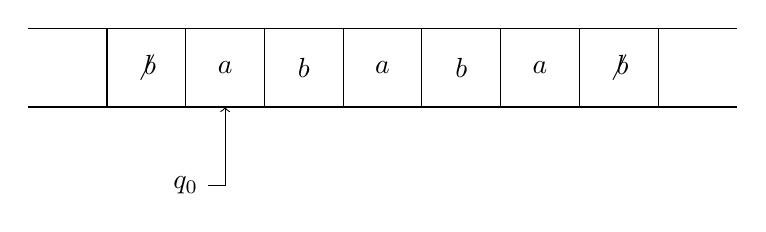
\begin{tikzpicture}
			\draw (0,0) -- (9,0);
			\draw (0,-1) -- (9,-1);
			
			\edef\i{1};
			\foreach \symb in {$\not b$,$a$,$b$,$a$,$b$,$a$,$\not b$} {
				\draw (\i,0) -- (\i,-1);
				\node at (\i+0.5,-0.5) {\symb};
				\pgfmathparse{\i+1}
				\xdef\i{\pgfmathresult}
			}
			\draw (\i,0) -- (\i,-1);
			
			\node (k) at (2,-2) {$q_0$};
			\draw (k) -- (2.5,-2);
			\draw[->] (2.5,-2) -- (2.5,-1);
			\end{tikzpicture}
		\end{center}
		\begin{center}
			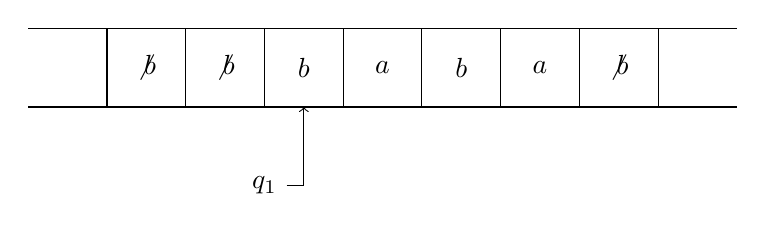
\begin{tikzpicture}
			\draw (0,0) -- (9,0);
			\draw (0,-1) -- (9,-1);
			
			\edef\i{1};
			\foreach \symb in {$\not b$,$\not b$,$b$,$a$,$b$,$a$,$\not b$} {
				\draw (\i,0) -- (\i,-1);
				\node at (\i+0.5,-0.5) {\symb};
				\pgfmathparse{\i+1}
				\xdef\i{\pgfmathresult}
			}
			\draw (\i,0) -- (\i,-1);
			
			\node (k) at (3,-2) {$q_1$};
			\draw (k) -- (3.5,-2);
			\draw[->] (3.5,-2) -- (3.5,-1);
			\end{tikzpicture}
		\end{center}
		\begin{center}
			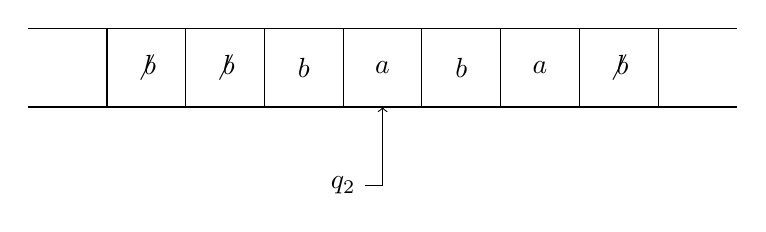
\begin{tikzpicture}
			\draw (0,0) -- (9,0);
			\draw (0,-1) -- (9,-1);
			
			\edef\i{1};
			\foreach \symb in {$\not b$,$\not b$,$b$,$a$,$b$,$a$,$\not b$} {
				\draw (\i,0) -- (\i,-1);
				\node at (\i+0.5,-0.5) {\symb};
				\pgfmathparse{\i+1}
				\xdef\i{\pgfmathresult}
			}
			\draw (\i,0) -- (\i,-1);
			
			\node (k) at (4,-2) {$q_2$};
			\draw (k) -- (4.5,-2);
			\draw[->] (4.5,-2) -- (4.5,-1);
			\end{tikzpicture}
		\end{center}
		Zustand verändert sich nicht, keine Ersetzungen finden statt, Lese-Schreibkopf bewegt sich nur nach rechts
		\begin{center}
			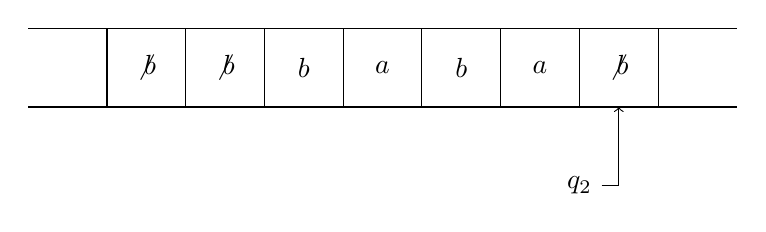
\begin{tikzpicture}
			\draw (0,0) -- (9,0);
			\draw (0,-1) -- (9,-1);
			
			\edef\i{1};
			\foreach \symb in {$\not b$,$\not b$,$b$,$a$,$b$,$a$,$\not b$} {
				\draw (\i,0) -- (\i,-1);
				\node at (\i+0.5,-0.5) {\symb};
				\pgfmathparse{\i+1}
				\xdef\i{\pgfmathresult}
			}
			\draw (\i,0) -- (\i,-1);
			
			\node (k) at (7,-2) {$q_2$};
			\draw (k) -- (7.5,-2);
			\draw[->] (7.5,-2) -- (7.5,-1);
			\end{tikzpicture}
		\end{center}
		\begin{center}
			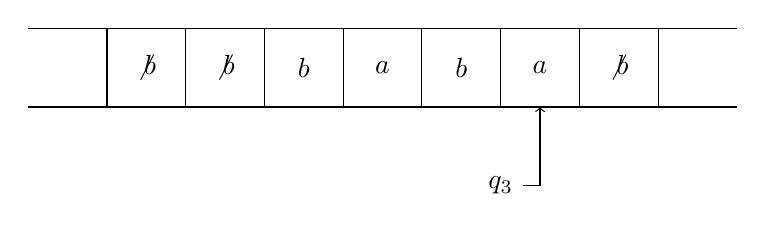
\begin{tikzpicture}
			\draw (0,0) -- (9,0);
			\draw (0,-1) -- (9,-1);
			
			\edef\i{1};
			\foreach \symb in {$\not b$,$\not b$,$b$,$a$,$b$,$a$,$\not b$} {
				\draw (\i,0) -- (\i,-1);
				\node at (\i+0.5,-0.5) {\symb};
				\pgfmathparse{\i+1}
				\xdef\i{\pgfmathresult}
			}
			\draw (\i,0) -- (\i,-1);
			
			\node (k) at (6,-2) {$q_3$};
			\draw (k) -- (6.5,-2);
			\draw[->] (6.5,-2) -- (6.5,-1);
			\end{tikzpicture}
		\end{center}
		\begin{center}
			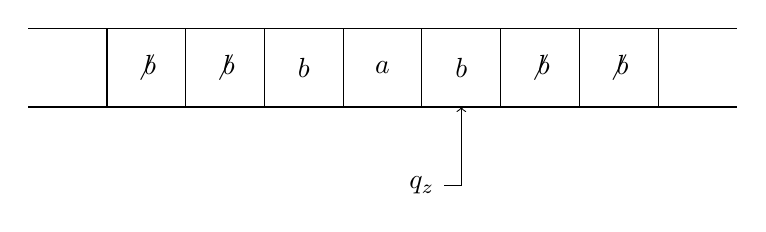
\begin{tikzpicture}
			\draw (0,0) -- (9,0);
			\draw (0,-1) -- (9,-1);
			
			\edef\i{1};
			\foreach \symb in {$\not b$,$\not b$,$b$,$a$,$b$,$\not b$,$\not b$} {
				\draw (\i,0) -- (\i,-1);
				\node at (\i+0.5,-0.5) {\symb};
				\pgfmathparse{\i+1}
				\xdef\i{\pgfmathresult}
			}
			\draw (\i,0) -- (\i,-1);
			
			\node (k) at (5,-2) {$q_z$};
			\draw (k) -- (5.5,-2);
			\draw[->] (5.5,-2) -- (5.5,-1);
			\end{tikzpicture}
		\end{center}
		Zustand verändert sich nicht, keine Ersetzungen finden statt, Lese-Schreibkopf bewegt sich nur nach links
		\begin{center}
			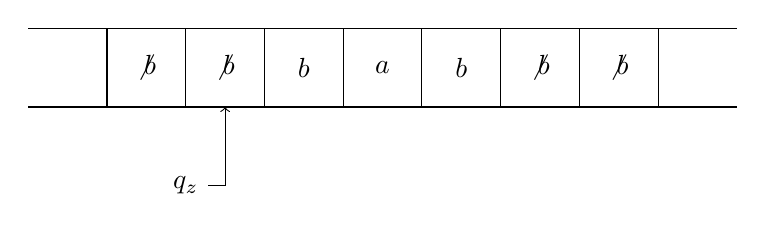
\begin{tikzpicture}
			\draw (0,0) -- (9,0);
			\draw (0,-1) -- (9,-1);
			
			\edef\i{1};
			\foreach \symb in {$\not b$,$\not b$,$b$,$a$,$b$,$\not b$,$\not b$} {
				\draw (\i,0) -- (\i,-1);
				\node at (\i+0.5,-0.5) {\symb};
				\pgfmathparse{\i+1}
				\xdef\i{\pgfmathresult}
			}
			\draw (\i,0) -- (\i,-1);
			
			\node (k) at (2,-2) {$q_z$};
			\draw (k) -- (2.5,-2);
			\draw[->] (2.5,-2) -- (2.5,-1);
			\end{tikzpicture}
		\end{center}
		\begin{center}
			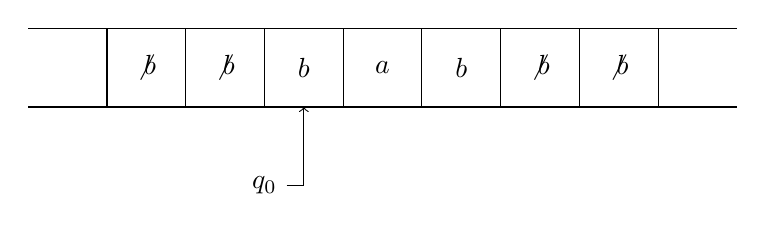
\begin{tikzpicture}
			\draw (0,0) -- (9,0);
			\draw (0,-1) -- (9,-1);
			
			\edef\i{1};
			\foreach \symb in {$\not b$,$\not b$,$b$,$a$,$b$,$\not b$,$\not b$} {
				\draw (\i,0) -- (\i,-1);
				\node at (\i+0.5,-0.5) {\symb};
				\pgfmathparse{\i+1}
				\xdef\i{\pgfmathresult}
			}
			\draw (\i,0) -- (\i,-1);
			
			\node (k) at (3,-2) {$q_0$};
			\draw (k) -- (3.5,-2);
			\draw[->] (3.5,-2) -- (3.5,-1);
			\end{tikzpicture}
		\end{center}
		\begin{center}
			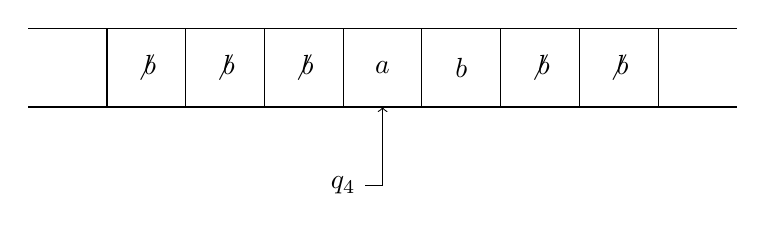
\begin{tikzpicture}
			\draw (0,0) -- (9,0);
			\draw (0,-1) -- (9,-1);
			
			\edef\i{1};
			\foreach \symb in {$\not b$,$\not b$,$\not b$,$a$,$b$,$\not b$,$\not b$} {
				\draw (\i,0) -- (\i,-1);
				\node at (\i+0.5,-0.5) {\symb};
				\pgfmathparse{\i+1}
				\xdef\i{\pgfmathresult}
			}
			\draw (\i,0) -- (\i,-1);
			
			\node (k) at (4,-2) {$q_4$};
			\draw (k) -- (4.5,-2);
			\draw[->] (4.5,-2) -- (4.5,-1);
			\end{tikzpicture}
		\end{center}
		\begin{center}
			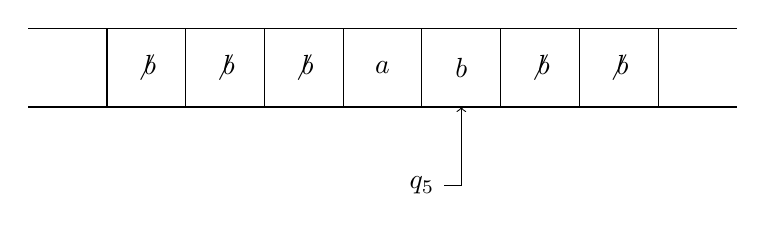
\begin{tikzpicture}
			\draw (0,0) -- (9,0);
			\draw (0,-1) -- (9,-1);
			
			\edef\i{1};
			\foreach \symb in {$\not b$,$\not b$,$\not b$,$a$,$b$,$\not b$,$\not b$} {
				\draw (\i,0) -- (\i,-1);
				\node at (\i+0.5,-0.5) {\symb};
				\pgfmathparse{\i+1}
				\xdef\i{\pgfmathresult}
			}
			\draw (\i,0) -- (\i,-1);
			
			\node (k) at (5,-2) {$q_5$};
			\draw (k) -- (5.5,-2);
			\draw[->] (5.5,-2) -- (5.5,-1);
			\end{tikzpicture}
		\end{center}
		\begin{center}
			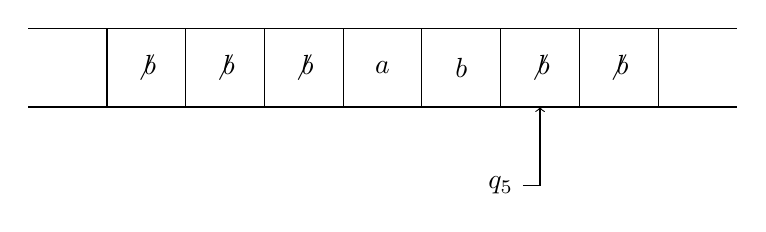
\begin{tikzpicture}
			\draw (0,0) -- (9,0);
			\draw (0,-1) -- (9,-1);
			
			\edef\i{1};
			\foreach \symb in {$\not b$,$\not b$,$\not b$,$a$,$b$,$\not b$,$\not b$} {
				\draw (\i,0) -- (\i,-1);
				\node at (\i+0.5,-0.5) {\symb};
				\pgfmathparse{\i+1}
				\xdef\i{\pgfmathresult}
			}
			\draw (\i,0) -- (\i,-1);
			
			\node (k) at (6,-2) {$q_5$};
			\draw (k) -- (6.5,-2);
			\draw[->] (6.5,-2) -- (6.5,-1);
			\end{tikzpicture}
		\end{center}
		\begin{center}
			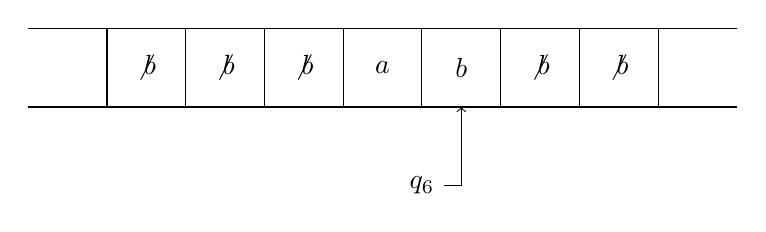
\begin{tikzpicture}
			\draw (0,0) -- (9,0);
			\draw (0,-1) -- (9,-1);
			
			\edef\i{1};
			\foreach \symb in {$\not b$,$\not b$,$\not b$,$a$,$b$,$\not b$,$\not b$} {
				\draw (\i,0) -- (\i,-1);
				\node at (\i+0.5,-0.5) {\symb};
				\pgfmathparse{\i+1}
				\xdef\i{\pgfmathresult}
			}
			\draw (\i,0) -- (\i,-1);
			
			\node (k) at (5,-2) {$q_6$};
			\draw (k) -- (5.5,-2);
			\draw[->] (5.5,-2) -- (5.5,-1);
			\end{tikzpicture}
		\end{center}
		\begin{center}
			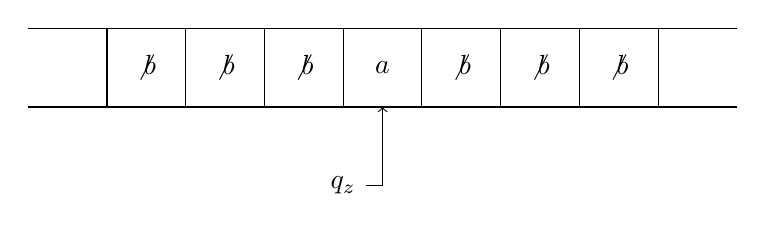
\begin{tikzpicture}
			\draw (0,0) -- (9,0);
			\draw (0,-1) -- (9,-1);
			
			\edef\i{1};
			\foreach \symb in {$\not b$,$\not b$,$\not b$,$a$,$\not b$,$\not b$,$\not b$} {
				\draw (\i,0) -- (\i,-1);
				\node at (\i+0.5,-0.5) {\symb};
				\pgfmathparse{\i+1}
				\xdef\i{\pgfmathresult}
			}
			\draw (\i,0) -- (\i,-1);
			
			\node (k) at (4,-2) {$q_z$};
			\draw (k) -- (4.5,-2);
			\draw[->] (4.5,-2) -- (4.5,-1);
			\end{tikzpicture}
		\end{center}
		\begin{center}
			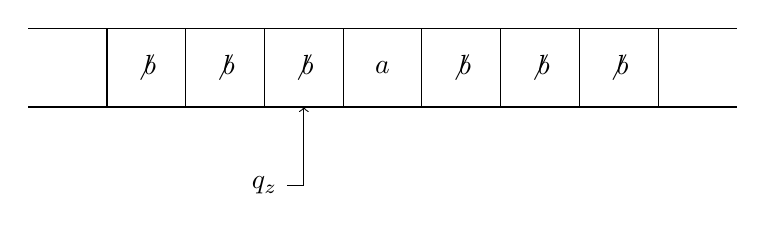
\begin{tikzpicture}
			\draw (0,0) -- (9,0);
			\draw (0,-1) -- (9,-1);
			
			\edef\i{1};
			\foreach \symb in {$\not b$,$\not b$,$\not b$,$a$,$\not b$,$\not b$,$\not b$} {
				\draw (\i,0) -- (\i,-1);
				\node at (\i+0.5,-0.5) {\symb};
				\pgfmathparse{\i+1}
				\xdef\i{\pgfmathresult}
			}
			\draw (\i,0) -- (\i,-1);
			
			\node (k) at (3,-2) {$q_z$};
			\draw (k) -- (3.5,-2);
			\draw[->] (3.5,-2) -- (3.5,-1);
			\end{tikzpicture}
		\end{center}
		\begin{center}
			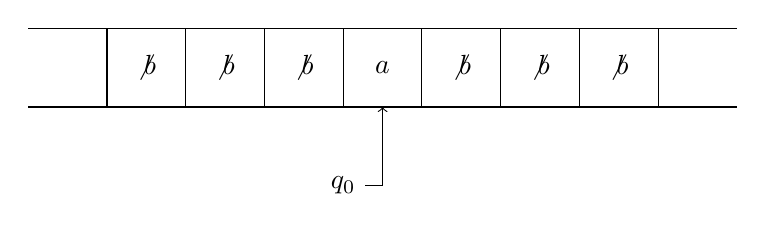
\begin{tikzpicture}
			\draw (0,0) -- (9,0);
			\draw (0,-1) -- (9,-1);
			
			\edef\i{1};
			\foreach \symb in {$\not b$,$\not b$,$\not b$,$a$,$\not b$,$\not b$,$\not b$} {
				\draw (\i,0) -- (\i,-1);
				\node at (\i+0.5,-0.5) {\symb};
				\pgfmathparse{\i+1}
				\xdef\i{\pgfmathresult}
			}
			\draw (\i,0) -- (\i,-1);
			
			\node (k) at (4,-2) {$q_0$};
			\draw (k) -- (4.5,-2);
			\draw[->] (4.5,-2) -- (4.5,-1);
			\end{tikzpicture}
		\end{center}
		\begin{center}
			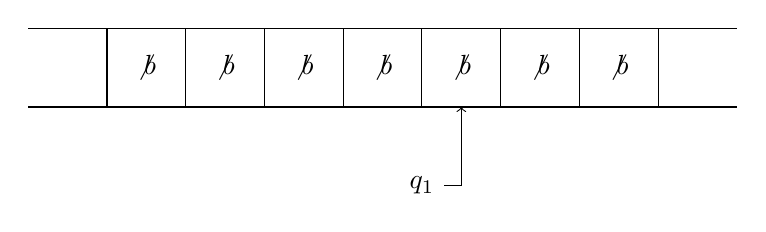
\begin{tikzpicture}
			\draw (0,0) -- (9,0);
			\draw (0,-1) -- (9,-1);
			
			\edef\i{1};
			\foreach \symb in {$\not b$,$\not b$,$\not b$,$\not b$,$\not b$,$\not b$,$\not b$} {
				\draw (\i,0) -- (\i,-1);
				\node at (\i+0.5,-0.5) {\symb};
				\pgfmathparse{\i+1}
				\xdef\i{\pgfmathresult}
			}
			\draw (\i,0) -- (\i,-1);
			
			\node (k) at (5,-2) {$q_1$};
			\draw (k) -- (5.5,-2);
			\draw[->] (5.5,-2) -- (5.5,-1);
			\end{tikzpicture}
		\end{center}
		\item Turingmaschine hält nicht an $\Rightarrow abaa\notin L(\mathcal{A})$
		\begin{center}
			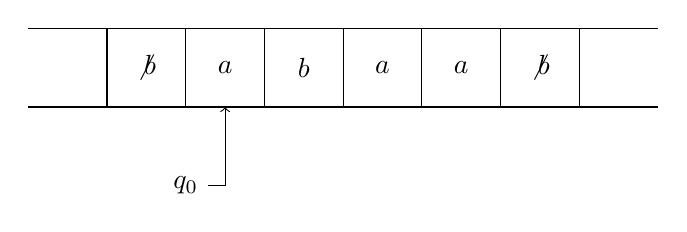
\begin{tikzpicture}
			\draw (0,0) -- (8,0);
			\draw (0,-1) -- (8,-1);
			
			\edef\i{1};
			\foreach \symb in {$\not b$,$a$,$b$,$a$,$a$,$\not b$} {
				\draw (\i,0) -- (\i,-1);
				\node at (\i+0.5,-0.5) {\symb};
				\pgfmathparse{\i+1}
				\xdef\i{\pgfmathresult}
			}
			\draw (\i,0) -- (\i,-1);
			
			\node (k) at (2,-2) {$q_0$};
			\draw (k) -- (2.5,-2);
			\draw[->] (2.5,-2) -- (2.5,-1);
			\end{tikzpicture}
		\end{center}
		\begin{center}
			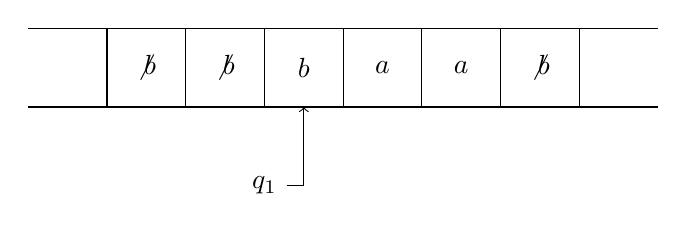
\begin{tikzpicture}
			\draw (0,0) -- (8,0);
			\draw (0,-1) -- (8,-1);
			
			\edef\i{1};
			\foreach \symb in {$\not b$,$\not b$,$b$,$a$,$a$,$\not b$} {
				\draw (\i,0) -- (\i,-1);
				\node at (\i+0.5,-0.5) {\symb};
				\pgfmathparse{\i+1}
				\xdef\i{\pgfmathresult}
			}
			\draw (\i,0) -- (\i,-1);
			
			\node (k) at (3,-2) {$q_1$};
			\draw (k) -- (3.5,-2);
			\draw[->] (3.5,-2) -- (3.5,-1);
			\end{tikzpicture}
		\end{center}
		\begin{center}
			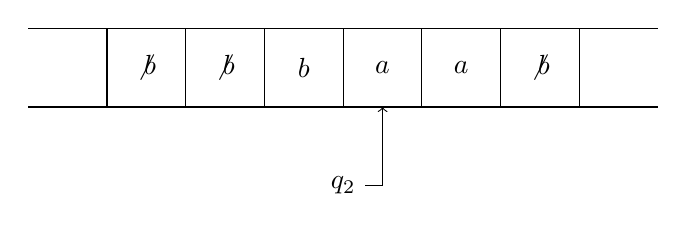
\begin{tikzpicture}
			\draw (0,0) -- (8,0);
			\draw (0,-1) -- (8,-1);
			
			\edef\i{1};
			\foreach \symb in {$\not b$,$\not b$,$b$,$a$,$a$,$\not b$} {
				\draw (\i,0) -- (\i,-1);
				\node at (\i+0.5,-0.5) {\symb};
				\pgfmathparse{\i+1}
				\xdef\i{\pgfmathresult}
			}
			\draw (\i,0) -- (\i,-1);
			
			\node (k) at (4,-2) {$q_2$};
			\draw (k) -- (4.5,-2);
			\draw[->] (4.5,-2) -- (4.5,-1);
			\end{tikzpicture}
		\end{center}
		Zustand verändert sich nicht, keine Ersetzungen finden statt, Lese-Schreibkopf bewegt sich nur nach rechts
		\begin{center}
			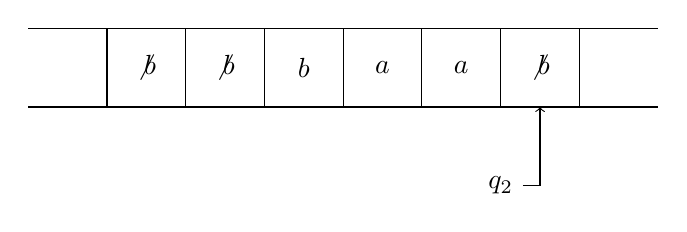
\begin{tikzpicture}
			\draw (0,0) -- (8,0);
			\draw (0,-1) -- (8,-1);
			
			\edef\i{1};
			\foreach \symb in {$\not b$,$\not b$,$b$,$a$,$a$,$\not b$} {
				\draw (\i,0) -- (\i,-1);
				\node at (\i+0.5,-0.5) {\symb};
				\pgfmathparse{\i+1}
				\xdef\i{\pgfmathresult}
			}
			\draw (\i,0) -- (\i,-1);
			
			\node (k) at (6,-2) {$q_2$};
			\draw (k) -- (6.5,-2);
			\draw[->] (6.5,-2) -- (6.5,-1);
			\end{tikzpicture}
		\end{center}
		\begin{center}
			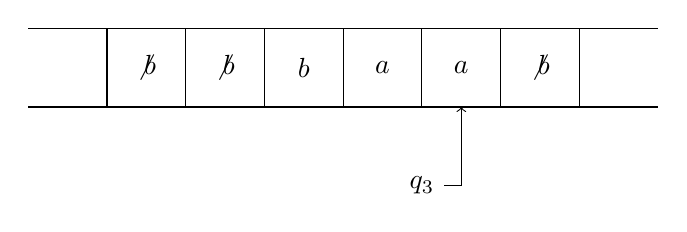
\begin{tikzpicture}
			\draw (0,0) -- (8,0);
			\draw (0,-1) -- (8,-1);
			
			\edef\i{1};
			\foreach \symb in {$\not b$,$\not b$,$b$,$a$,$a$,$\not b$} {
				\draw (\i,0) -- (\i,-1);
				\node at (\i+0.5,-0.5) {\symb};
				\pgfmathparse{\i+1}
				\xdef\i{\pgfmathresult}
			}
			\draw (\i,0) -- (\i,-1);
			
			\node (k) at (5,-2) {$q_3$};
			\draw (k) -- (5.5,-2);
			\draw[->] (5.5,-2) -- (5.5,-1);
			\end{tikzpicture}
		\end{center}
		\begin{center}
			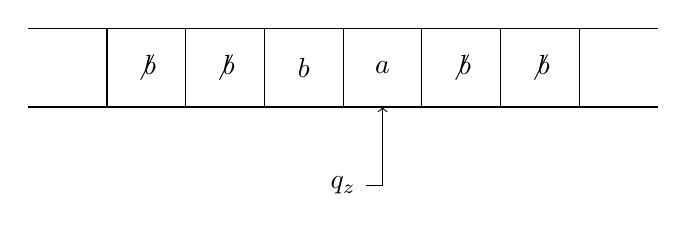
\begin{tikzpicture}
			\draw (0,0) -- (8,0);
			\draw (0,-1) -- (8,-1);
			
			\edef\i{1};
			\foreach \symb in {$\not b$,$\not b$,$b$,$a$,$\not b$,$\not b$} {
				\draw (\i,0) -- (\i,-1);
				\node at (\i+0.5,-0.5) {\symb};
				\pgfmathparse{\i+1}
				\xdef\i{\pgfmathresult}
			}
			\draw (\i,0) -- (\i,-1);
			
			\node (k) at (4,-2) {$q_z$};
			\draw (k) -- (4.5,-2);
			\draw[->] (4.5,-2) -- (4.5,-1);
			\end{tikzpicture}
		\end{center}
		Zustand verändert sich nicht, keine Ersetzungen finden statt, Lese-Schreibkopf bewegt sich nur nach links
		\begin{center}
			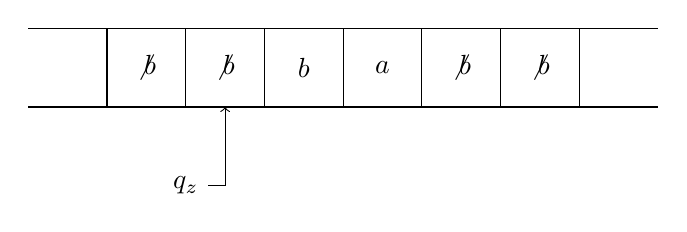
\begin{tikzpicture}
			\draw (0,0) -- (8,0);
			\draw (0,-1) -- (8,-1);
			
			\edef\i{1};
			\foreach \symb in {$\not b$,$\not b$,$b$,$a$,$\not b$,$\not b$} {
				\draw (\i,0) -- (\i,-1);
				\node at (\i+0.5,-0.5) {\symb};
				\pgfmathparse{\i+1}
				\xdef\i{\pgfmathresult}
			}
			\draw (\i,0) -- (\i,-1);
			
			\node (k) at (2,-2) {$q_z$};
			\draw (k) -- (2.5,-2);
			\draw[->] (2.5,-2) -- (2.5,-1);
			\end{tikzpicture}
		\end{center}
		\begin{center}
			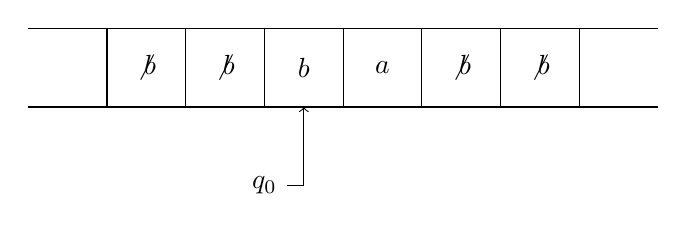
\begin{tikzpicture}
			\draw (0,0) -- (8,0);
			\draw (0,-1) -- (8,-1);
			
			\edef\i{1};
			\foreach \symb in {$\not b$,$\not b$,$b$,$a$,$\not b$,$\not b$} {
				\draw (\i,0) -- (\i,-1);
				\node at (\i+0.5,-0.5) {\symb};
				\pgfmathparse{\i+1}
				\xdef\i{\pgfmathresult}
			}
			\draw (\i,0) -- (\i,-1);
			
			\node (k) at (3,-2) {$q_0$};
			\draw (k) -- (3.5,-2);
			\draw[->] (3.5,-2) -- (3.5,-1);
			\end{tikzpicture}
		\end{center}
		\begin{center}
			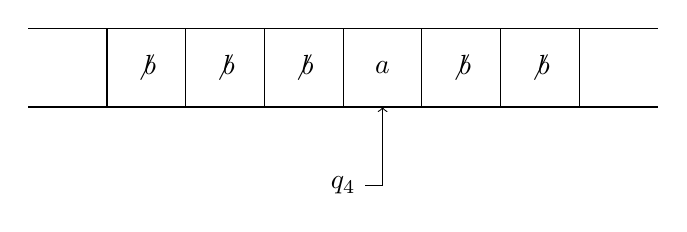
\begin{tikzpicture}
			\draw (0,0) -- (8,0);
			\draw (0,-1) -- (8,-1);
			
			\edef\i{1};
			\foreach \symb in {$\not b$,$\not b$,$\not b$,$a$,$\not b$,$\not b$} {
				\draw (\i,0) -- (\i,-1);
				\node at (\i+0.5,-0.5) {\symb};
				\pgfmathparse{\i+1}
				\xdef\i{\pgfmathresult}
			}
			\draw (\i,0) -- (\i,-1);
			
			\node (k) at (4,-2) {$q_4$};
			\draw (k) -- (4.5,-2);
			\draw[->] (4.5,-2) -- (4.5,-1);
			\end{tikzpicture}
		\end{center}
		\begin{center}
			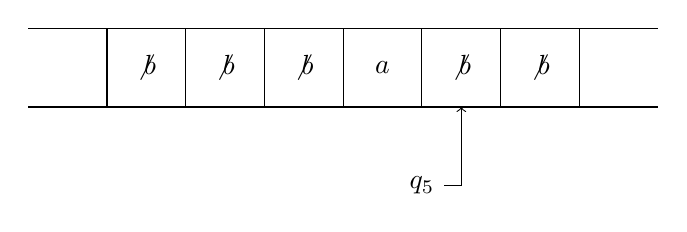
\begin{tikzpicture}
			\draw (0,0) -- (8,0);
			\draw (0,-1) -- (8,-1);
			
			\edef\i{1};
			\foreach \symb in {$\not b$,$\not b$,$\not b$,$a$,$\not b$,$\not b$} {
				\draw (\i,0) -- (\i,-1);
				\node at (\i+0.5,-0.5) {\symb};
				\pgfmathparse{\i+1}
				\xdef\i{\pgfmathresult}
			}
			\draw (\i,0) -- (\i,-1);
			
			\node (k) at (5,-2) {$q_5$};
			\draw (k) -- (5.5,-2);
			\draw[->] (5.5,-2) -- (5.5,-1);
			\end{tikzpicture}
		\end{center}
		\begin{center}
			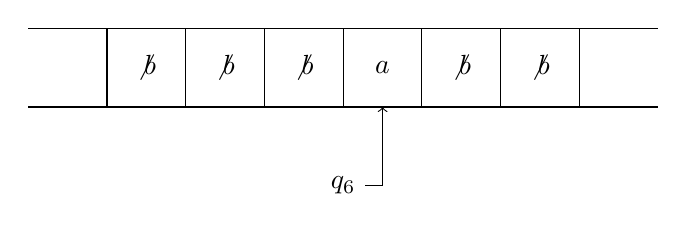
\begin{tikzpicture}
			\draw (0,0) -- (8,0);
			\draw (0,-1) -- (8,-1);
			
			\edef\i{1};
			\foreach \symb in {$\not b$,$\not b$,$\not b$,$a$,$\not b$,$\not b$} {
				\draw (\i,0) -- (\i,-1);
				\node at (\i+0.5,-0.5) {\symb};
				\pgfmathparse{\i+1}
				\xdef\i{\pgfmathresult}
			}
			\draw (\i,0) -- (\i,-1);
			
			\node (k) at (4,-2) {$q_6$};
			\draw (k) -- (4.5,-2);
			\draw[->] (4.5,-2) -- (4.5,-1);
			\end{tikzpicture}
		\end{center}
		\begin{center}
			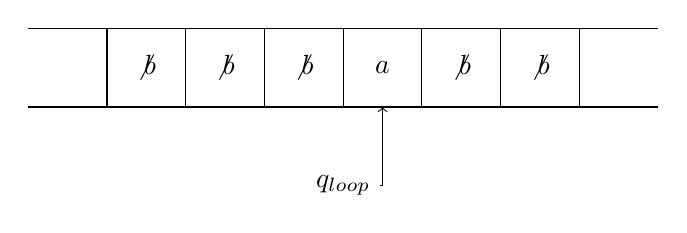
\begin{tikzpicture}
			\draw (0,0) -- (8,0);
			\draw (0,-1) -- (8,-1);
			
			\edef\i{1};
			\foreach \symb in {$\not b$,$\not b$,$\not b$,$a$,$\not b$,$\not b$} {
				\draw (\i,0) -- (\i,-1);
				\node at (\i+0.5,-0.5) {\symb};
				\pgfmathparse{\i+1}
				\xdef\i{\pgfmathresult}
			}
			\draw (\i,0) -- (\i,-1);
			
			\node (k) at (4,-2) {$q_{loop}$};
			\draw (k) -- (4.5,-2);
			\draw[->] (4.5,-2) -- (4.5,-1);
			\end{tikzpicture}
		\end{center}
		\item $q_0$: Löschen des ersten Buchstabens und entscheiden $q_1-q_3$-Zweig oder $q_4-q_6$-Zweig \\
		$q_1+q_2$: zum Ende des Wortes gehen ($q_1$ sorgt dafür, dass eine Möglichkeit für die Turingmaschine gibt anzuhalten, weil $\not b$ in $q_1$ nicht behandelt wird) \\
		$q_3$: letzten Buchstaben des Wortes lesen: $a\Rightarrow q_z$, $b\Rightarrow q_{loop}$ \\
		$q_4$-$q_6$: machen das selbe wie $q_1$-$q_3$ nur für $b$ \\
		$q_z$: zum Anfang des (verkürzten) Wortes gehen \\
		$q_{loop}$: Endlosschleife, um Turingmaschine am laufen zu halten
		\item Palindrome über $\{a,b\}$
	\end{enumerate}
	
	\section*{Aufgabe 10.2}

	$\mathcal{A}=(\{q_0\},\{a,b\},\{a,b,\not b\},q_0,\delta)$ mit $\delta$
	\begin{center}
		\begin{tabular}{cccccc}
			$q_0$ & $a$ & $\to$ & $a$ & $n$ & $q_0$ \\
			$q_0$ & $b$ & $\to$ & $b$ & $n$ & $q_0$
		\end{tabular}
	\end{center}

	\section*{Aufgabe 10.3}
	
	Idee:
	\begin{center}
		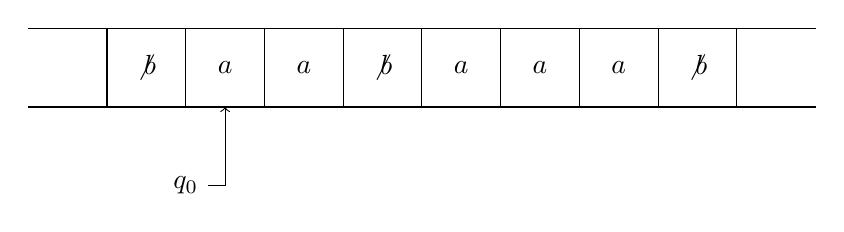
\begin{tikzpicture}
		\draw (0,0) -- (10,0);
		\draw (0,-1) -- (10,-1);
		
		\edef\i{1};
		\foreach \symb in {$\not b$,$a$,$a$,$\not b$,$a$,$a$,$a$,$\not b$} {
			\draw (\i,0) -- (\i,-1);
			\node at (\i+0.5,-0.5) {\symb};
			\pgfmathparse{\i+1}
			\xdef\i{\pgfmathresult}
		}
		\draw (\i,0) -- (\i,-1);
		
		\node (k) at (2,-2) {$q_{0}$};
		\draw (k) -- (2.5,-2);
		\draw[->] (2.5,-2) -- (2.5,-1);
		\end{tikzpicture}
	\end{center}
	\begin{center}
		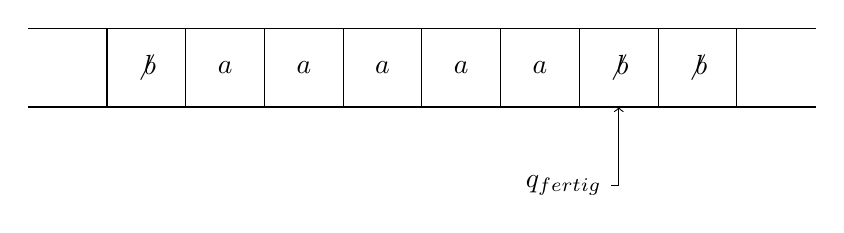
\begin{tikzpicture}
		\draw (0,0) -- (10,0);
		\draw (0,-1) -- (10,-1);
		
		\edef\i{1};
		\foreach \symb in {$\not b$,$a$,$a$,$a$,$a$,$a$,$\not b$,$\not b$} {
			\draw (\i,0) -- (\i,-1);
			\node at (\i+0.5,-0.5) {\symb};
			\pgfmathparse{\i+1}
			\xdef\i{\pgfmathresult}
		}
		\draw (\i,0) -- (\i,-1);
		
		\node (k) at (6.8,-2) {$q_{fertig}$};
		\draw (k) -- (7.5,-2);
		\draw[->] (7.5,-2) -- (7.5,-1);
		\end{tikzpicture}
	\end{center}

	$\mathcal{A}=(\{q_0,q_1,q_2,q_{fertig}\},\{a\},\{a,\not b\},q_0,\delta)$ mit $\delta$
	\begin{center}
		\begin{tabular}{cccccc}
			$q_0$ & $a$ & $\to$ & $a$ & $r$ & $q_0$ \\
			$q_0$ & $\not b$ & $\to$ & $a$ & $r$ & $q_1$ \\
			\hline
			$q_1$ & $a$ & $\to$ & $a$ & $r$ & $q_1$ \\
			$q_1$ & $\not b$ & $\to$ & $\not b$ & $l$ & $q_2$ \\
			\hline
			$q_2$ & $a$ & $\to$ & $\not b$ & $n$ & $q_{fertig}$ \\
			\hline
			$q_{fertig}$ & $a$ & $\to$ & $a$ & $l$ & $q_{fertig}$
		\end{tabular}
	\end{center}
\end{document}